\documentclass[jou,apacite, 10px]{apa6}
\usepackage{listings}
\usepackage{courier}
\usepackage{CJKutf8}
\usepackage[shortlabels]{enumitem}
\lstset{basicstyle=\small\ttfamily,breaklines=true}
\lstset{frame=single}
\makeatletter
\newcommand*{\rom}[1]{\expandafter\@slowromancap\romannumeral #1@}
\makeatother
\title{Classify a book's category based on its title}
\shorttitle{Book classification using book titles}

\twoauthors{Yunkai Wang}{Jules Kuehn}
\twoaffiliations{Carleton University, School of Computer Science}{Carleton University, School of Computer Science}

\abstract{Recently Convolutional Neural Networks (CNN) have been well-studied and be shown that they can archive incredible results on tasks like sentence classification (Kim, 2014; Zhang and Wallace, 2015). An interesting topic that has been studied is if we can categorize a book based on its cover picture (Iwana et al., 2016). "However, classification of books based on the cover image is a difficult task." (Iwana et al., 2016, p. 6). As being said, relationship between the book's cover image and its category does exist, but it's hard to to classify using a CNN as many books have a misleading cover images. Based on the idea of categorizing book, we conduct this experiment to see if we can use CNN to learn the potential relationship between a book's title and its categories. For this project, we experiment how well this task can be performed with different model setups and layers (Britz, 2015) using matrices that represent the titles as input(Mikolov et al., 2013; Karani, 2018; Britz, 2015).}

\leftheader{Jules, Yunkai}

\begin{document}
\maketitle    
                        
\section{\rom{1}. Introduction}
Book titles will given the reader a first impression of what the book may be about, and most of the time, a good book title will attract more readers from buying and reading the book, it makes the book different from other books (Peterson, 2018). But what does the book title really tells you? What can you say about the book by simply looking at the book title? If a title contains the word 'calendar', then most likely people will all agree that it's a calendar, but what if the book title doesn't contain a specific word that reveals its category, like if you are given the book title 'The Three-Body Problem' with knowing this book before, how will you categorize the book? Will the book title be sufficient for a CNN that has been pre-trained with titles and categories be able to detect that book as a science friction, or will the CNN think that it's a physics book? This is a very interesting question to ask, and that's why we conduct this experiment, to see if the computers are able to learn the potential relationship between a book's title and its category using CNN.

\section{\rom{2}. Background/Related work}

\subsection{Dateset}
The \textit{Data Mining} is a dataset that can be found on \textit{Github.com}, and it's made published by the researchers who conducted the experiment on testing the relationship between a book's cover image and its category (Iwana et al., 2016; uchidalab, 2018). The set consists of detailed information of $207572$ books from $32$ different categories. Some of the books are easy to classify, like 'calendar' and 'law', which are not similar to the other categories, or they contain some specific keyword among most books from the same category. However, many categories are pairwise similar, like 'Christian Books and Bibles' and 'Religion and Spirituality', these categories are the difficult part for the CNN to correctly classify. The dataset is not automatically splitted into training set and test set, so we use \textit{sklearn} library to split the data.

\subsection{Loading and transforming the data}
Here are the list of things we did to load the dataset:

\rule{0pt}{4ex}  1. First we load all the original data line by line, and for each line, we extract the book title and its category, as those are the only things that we are feeding to our neural network.

\rule{0pt}{4ex}  2. Since most titles are of different length, and the maximum title length is $96$. We could expand the titles so that they all have length $96$. However, as Figure $1$ shows, most of titles have length less than $26$, only several titles have length $>26$. Therefore, we choose the maximum length to be $26$ instead of $96$. We used \textit{pad\_sequence} function from keras library to accomplish the task, which simply appends $0$ to the end of the titles that are shorter than the given length, and cut-off those long titles after $26$ words.

\begin{figure}[h!]
\captionsetup{justification=centering}
     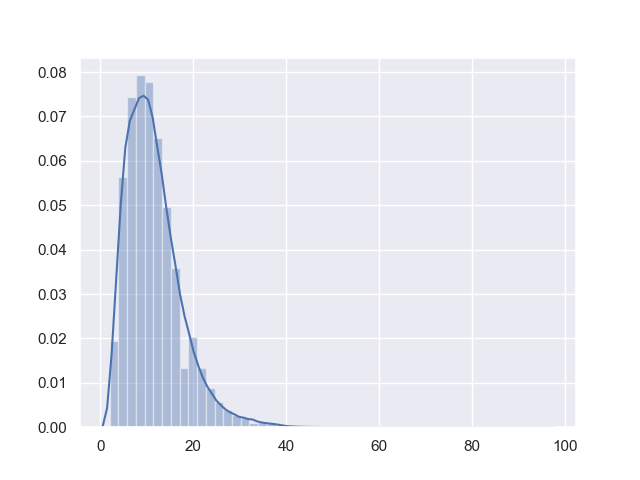
\includegraphics[width=0.5\textwidth]{images/title_lengths}
     \caption{Distributions of title lengths}
\end{figure}

\rule{0pt}{4ex}  3. With the help of \textit{train\_test\_split} function, we split the training data and testing data by having a testing data of size $10\%$ of the original dataset.

\rule{0pt}{4ex}  4. We convert the titles into matrices that can represent these titles, more details about this can be found in the 'Representing titles using matrices' section.

\subsection{Libraries}
In this project, we used the following libraries to avoid re-writing a lot of the codes that are not so important for the context of this experiment:

\begin{itemize}
\item keras: We used keras library a lot, like the data preprocessing functions and the functions that create the layers automatically.
\item sklearn: We used sklearn to split the training and testing dataset, and the TSNE function to plot the categories on a 2D graph.
\item tensorflow: Tensorflow was originally used in mlp.py and cnn.py files, and we used the models defined in those files to see how they perform on this task.
\end{itemize}

\subsection{Representing titles using matrices}
In order to apply CNNs to natural language processing (NLP) related tasks, the input are the words or sentences that are represented as matrices (Britz, 2015). Typically, we can use one of the two following mechanisms to represent the titles:
\begin{itemize}
\item Word embeddings: Using \textit{word2vec}("Word2vec", 2018) or \textit{GloVe}("GloVe: Global Vectors for Word Representation", 2014) to generate low-rank approximation of these titles (Karani, 2018).
\item One-hot: Convert the words into unique indices that represent these words, so each title becomes a vector of indices. This can be done using the \textit{one\_hot} function that is available in \textit{keras} library.
\end{itemize}

\section{\rom{3}. Problem Statement}

We want computers to be able to handle the categorization tasks for books based on book titles, such that in the future, the computer will be able to auto-categorize a new book given only its title, which will be faster than manually categorizing the books. It's almost impossible to manually design a rule-based program, that will handle the categorization problem nicely and accurately. The titles and the categories don't have an obvious relationship which we can use to linearly separate the titles into categories, there may be infinitely many potential relationships. However, if we success with our experiment, then we can use CNN to learn the underlying relationship between the titles and the categories, and the CNN will achieve a high accuracy in the categorization task.

\section{\rom{4}. Model}
We began with 2 naive implementations, in which each "word vector" was an arbitrary unique integer. Each title is then a vector of these integers (one for each word), zero padded to the length of the longest title (96 words). This representation of the titles has little semantic value as the integers representing the words are arbitrary.\\
% Insert diagram of naive model
The first model (NaiveMLP) was a fully connected MLP with the following configuration. Output size of each layer is indicated in parentheses.

\begin{itemize}
    \item Input (96)
    \item FC Sigmoid (625)
    \item FC Sigmoid (300)
    \item FC Softmax (32)
\end{itemize}\rule{0pt}{4ex}
The second model (NaiveCNN) was based on a good model for the CIFAR-10 classification.

\begin{itemize}
    \item Input (96,1)
    \item Conv ReLU: 3 kernel, 1 stride (96,32)
    \item Conv ReLU: 3 kernel, 1 stride (96,32)
    \item Max pool: 2 kernel, 2 stride (48,32)
    \item Dropout: pKeep 0.8 (48,32)
    \item Conv ReLU: 3 kernel, 1 stride (48,64)
    \item Max pool: 2 kernel, 2 stride (24,64)
    \item Conv ReLU: 3 kernel, 1 stride (24,64)
    \item Max pool: 24 kernel, 24 stride (1,64)
    \item Dropout: pKeep 0.8 (1,64)
    \item Output Softmax (32)
\end{itemize}\rule{0pt}{4ex}
A better word representation is to embed each word in a n-dimensional space, where the position of each word reflects its meaning in relation to the other words. Each word is then represented by a dense vector of length n, with similar words having similar vectors. Similarity between words is inferred from context. Many pre-trained embeddings are available, trained through Word2Vec or GloVe on datasets pulled from Wikipedia, Twitter, or other sources. An embedding can also be trained from scratch, or initialized to a pre-trained dataset then trained further. We compare these three approaches.\\
The first embedding model (EmbedTrain) trained the embeddings from scratch, using only the book titles from the training set. Note that we truncated the titles from a maximum of 96 words to 26 words. We chose 32 for the embedding dimension, based on the rule of the thumb that the embedding should be the fourth root of the vocabulary size. There were roughly 70,000 words in the training dataset, which suggest that the embedding dimension should be 16, but we found that 32 offered a slight improvement in practice.

\begin{itemize}
    \item Input (26, 1)
    \item Embedding (26, 32)
    \item Flatten (832)
    \item Dropout (832)
    \item Output Softmax (32)
\end{itemize}
For each of the three embedding models, we also tested 2 variations to compare the performance of MLP vs CNN on the title embeddings. The first variation (Embed<Model>\_FC) adds a single fully connected (FC) layer:\\
\begin{itemize}
    \item Input (26, 1)
    \item Embedding (26, 32)
    \item Flatten (832)
    \item Dropout (832)
    \item FC ReLU (512)
    \item Dropout (512)
    \item Output Softmax (32)
\end{itemize}\rule{0pt}{4ex}
The second variation (Embed<Model>\_CNN) adds a single convolutional layer, followed by maxpool over the entire length:

\begin{itemize}
    \item Input (26, 1)
    \item Embedding (26, 32)
    \item Conv ReLU: 3 kernel, 1 stride (24, 512)
    \item Max pool: 24 kernel, 24 stride (1, 512)
    \item Flatten (512)
    \item Dropout (512)
    \item Output Softmax (32)
\end{itemize}
The second embedding model (EmbedGloveFixed) loaded 400,000 pre-trained 100-dimensional word-vectors from the GloVe.6B dataset. These word vectors were trained on Wikipedia and Gigaword, a newswire dataset. The model is identical to EmbedTrain except that the embeddings are pre-trained and fixed, with the embedding dimension increased to 100.\\
The third embedding model (EmbedGloveTrain) is identical to EmbedTrain except that the embeddings are initialized to the GloVe dataset as seen in EmbedGloveFixed. Embeddings are then retrained on the book titles.

\section{\rom{4}. Implementation}
The naive models were implemented using the course-provided cnn.py and mlp.py code. All other models were implemented in Keras, in which the code for the model is extremely concise:\\
\lstinputlisting{code/kerasModel.py}

\section{\rom{5}. Experiment}
We did a couple of experiments using different models and configurations. Here is a detailed list and explanation of these experiments.

\section{\rom{6}. Conclusion}
In this project, we experimented using different neural network models to categorize book based on its title, and we archived a better result compared with the accuracies if the neural network judge the book based on its cover image (Iwana et al.). We have shown that with word embedding and a very simple CNN, we are able to categorize the books accurately, even though it's not categorizing well for some of the categories. However, since the neural network is very small, we are able to train the network within a reasonable short time, which makes it possible to train the network with a larger dataset in order to improve the result, especially feeding more training datas for those similar categories. For future improvement, we can try to make the CNN more complicated, or finding a new neural network model that is better at this job. but that will definitely make it harder to train the network with large data set because of the computational complexity. Another possibility to improve the result is to filter out some of the confusion words, or misleading words among the titles, where these words are the most common words that will cause a book title to be incorrectly categorized, but that's beyond the scope of this project as that requires a lot more data pre-processing and experiments on which set of words we should filter out in order to improve the result.

 The \textit{Data Mining} dataset is an interesting dataset to be working on, as it provides the capability to conducting many different possible classification experiments, like the relationship between a book title and the book author, etc. However, if the original dataset can provide a typical sentence from each book (like the first sentence from the book or the best sentence from the book), then we can conduct even more interesting experiments. Also, it will be helpful if people can enrich that dataset with more books that belong those small sized categories like Education \& training, which will definitely improve the classification accuracy of our model, and possibly the others.

\section{References}
\begin{enumerate}[(1)]
\item Britz, D. (2015a, November 7). Understanding Convolutional Neural Networks for NLP. Retrieved December 11, 2018, from http://www.wildml.com/2015/11/understanding-convolutional-neural-networks-for-nlp/
\item Britz, D. (2015b, December 11). Implementing a CNN for Text Classification in TensorFlow. Retrieved December 11, 2018, from http://www.wildml.com/2015/12/implementing-a-cnn-for-text-classification-in-tensorflow/
\item GloVe: Global Vectors for Word Representation. (n.d.). Retrieved December 15, 2018, from https://nlp.stanford.edu/projects/glove/
\item Iwana, B. K., Rizvi, S. T. R., Ahmed, S., Dengel, A., \& Uchida, S. (2016). Judging a Book By its Cover. ArXiv:1610.09204 [Cs]. Retrieved from http://arxiv.org/abs/1610.09204
\item Karani, D. (2018, September 1). Introduction to Word Embedding and Word2Vec. Retrieved December 11, 2018, from https://towardsdatascience.com/introduction-to-word-embedding-and-word2vec-652d0c2060fa
\item Kim, Y. (2014). Convolutional Neural Networks for Sentence Classification. ArXiv:1408.5882 [Cs]. Retrieved from http://arxiv.org/abs/1408.5882
Mikolov, T., Chen, K., Corrado, G., \& Dean, J. (2013). Efficient Estimation of Word Representations in Vector Space. ArXiv:1301.3781 [Cs]. Retrieved from http://arxiv.org/abs/1301.3781
\item Peterson, V. (n.d.). How to Write an Effective Book Title. Retrieved December 15, 2018, from https://www.thebalancecareers.com/how-to-write-a-book-title-insights-and-examples-2799918
\item This dataset contains 207,572 books from the Amazon.com, Inc. marketplace.: uchidalab/book-dataset. (2018). Python, \begin{CJK}{UTF8}{min}九州大学 ヒューマンインタフェース研究室\end{CJK}. Retrieved from https://github.com/uchidalab/book-dataset (Original work published 2017)
\item Word2vec. (2018). In Wikipedia. Retrieved from https://en.wikipedia.org/w/index.php?title=Word2vec\& oldid=869116438
\item Zhang, Y., \& Wallace, B. (2015). A Sensitivity Analysis of (and Practitioners’ Guide to) Convolutional Neural Networks for Sentence Classification. ArXiv:1510.03820 [Cs]. Retrieved from http://arxiv.org/abs/1510.03820
\end{enumerate}


\end{document}
